\documentclass[12pt,a4paper]{article}
\usepackage[utf8]{inputenc}
\usepackage[spanish]{babel}
\usepackage{amsmath}
\usepackage{amsfonts}
\usepackage{amssymb}
\usepackage{graphicx}
\usepackage{kpfonts}
\usepackage[left=2cm,right=2cm,top=2cm,bottom=2cm]{geometry}
\title{EV 2-6 CONSTRUIR AMPLIFICADOR DE POTENCIA CON CONEXION DARLINGTON

\includegraphics [scale=1]{imagenes/UPZMG.png} 
\author{Giovanni Daniel Ruiz Tinoco\\
Alan Antonio Muñoz Juarez\\
\small Sistemas electrónicos de interfaz\\
  \small Universidad Politécnica de la zona metropolitana de Guadalajara\\
  \small 4-B \\
  \small Ing. Mecatrónica\\
\centering
}
}
\begin{document}
\maketitle
\newpage
\begin{center}
\section {MARCO TEÓRICO}
\end{center}
\subsection{¿Qué es un Transistor Darlington?}
\begin{flushleft}
El transistor Darlington es un tipo especial de transistor que tiene una muy alta ganancia de corriente. Está compuesto internamente por dos transistores bipolares comunes que se conectan es cascada, como se muestra en el siguiente gráfico. \linebreak
\end{flushleft}
\begin{center}
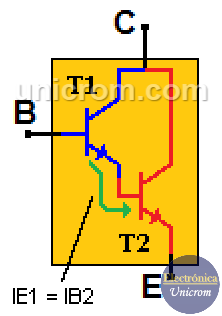
\includegraphics[scale=0.8]{imagenes/tiris.jpg} \linebreak 
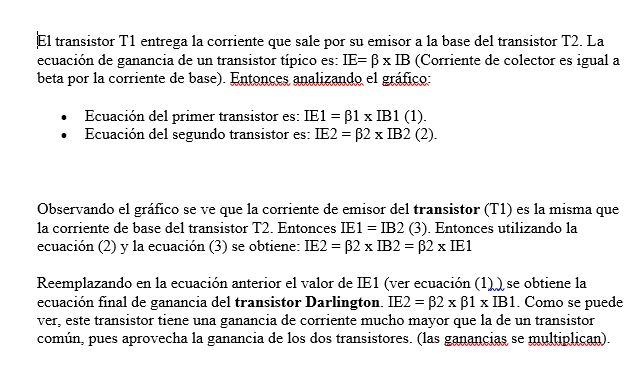
\includegraphics[scale=1]{imagenes/tira.jpg} \linebreak 
\end{center}
\newpage
\section{Materiales para la práctica}
\begin{flushleft}
-1 Transistor Darlington Tip 112\\
-1 LDR\\
-1 Resistencias \\
-1 POT 100k\\
-1 Led 
- Relés
Realice la simulaciones y los circuitos del siguientes esquemas:\\
\end{flushleft}
\begin{center}
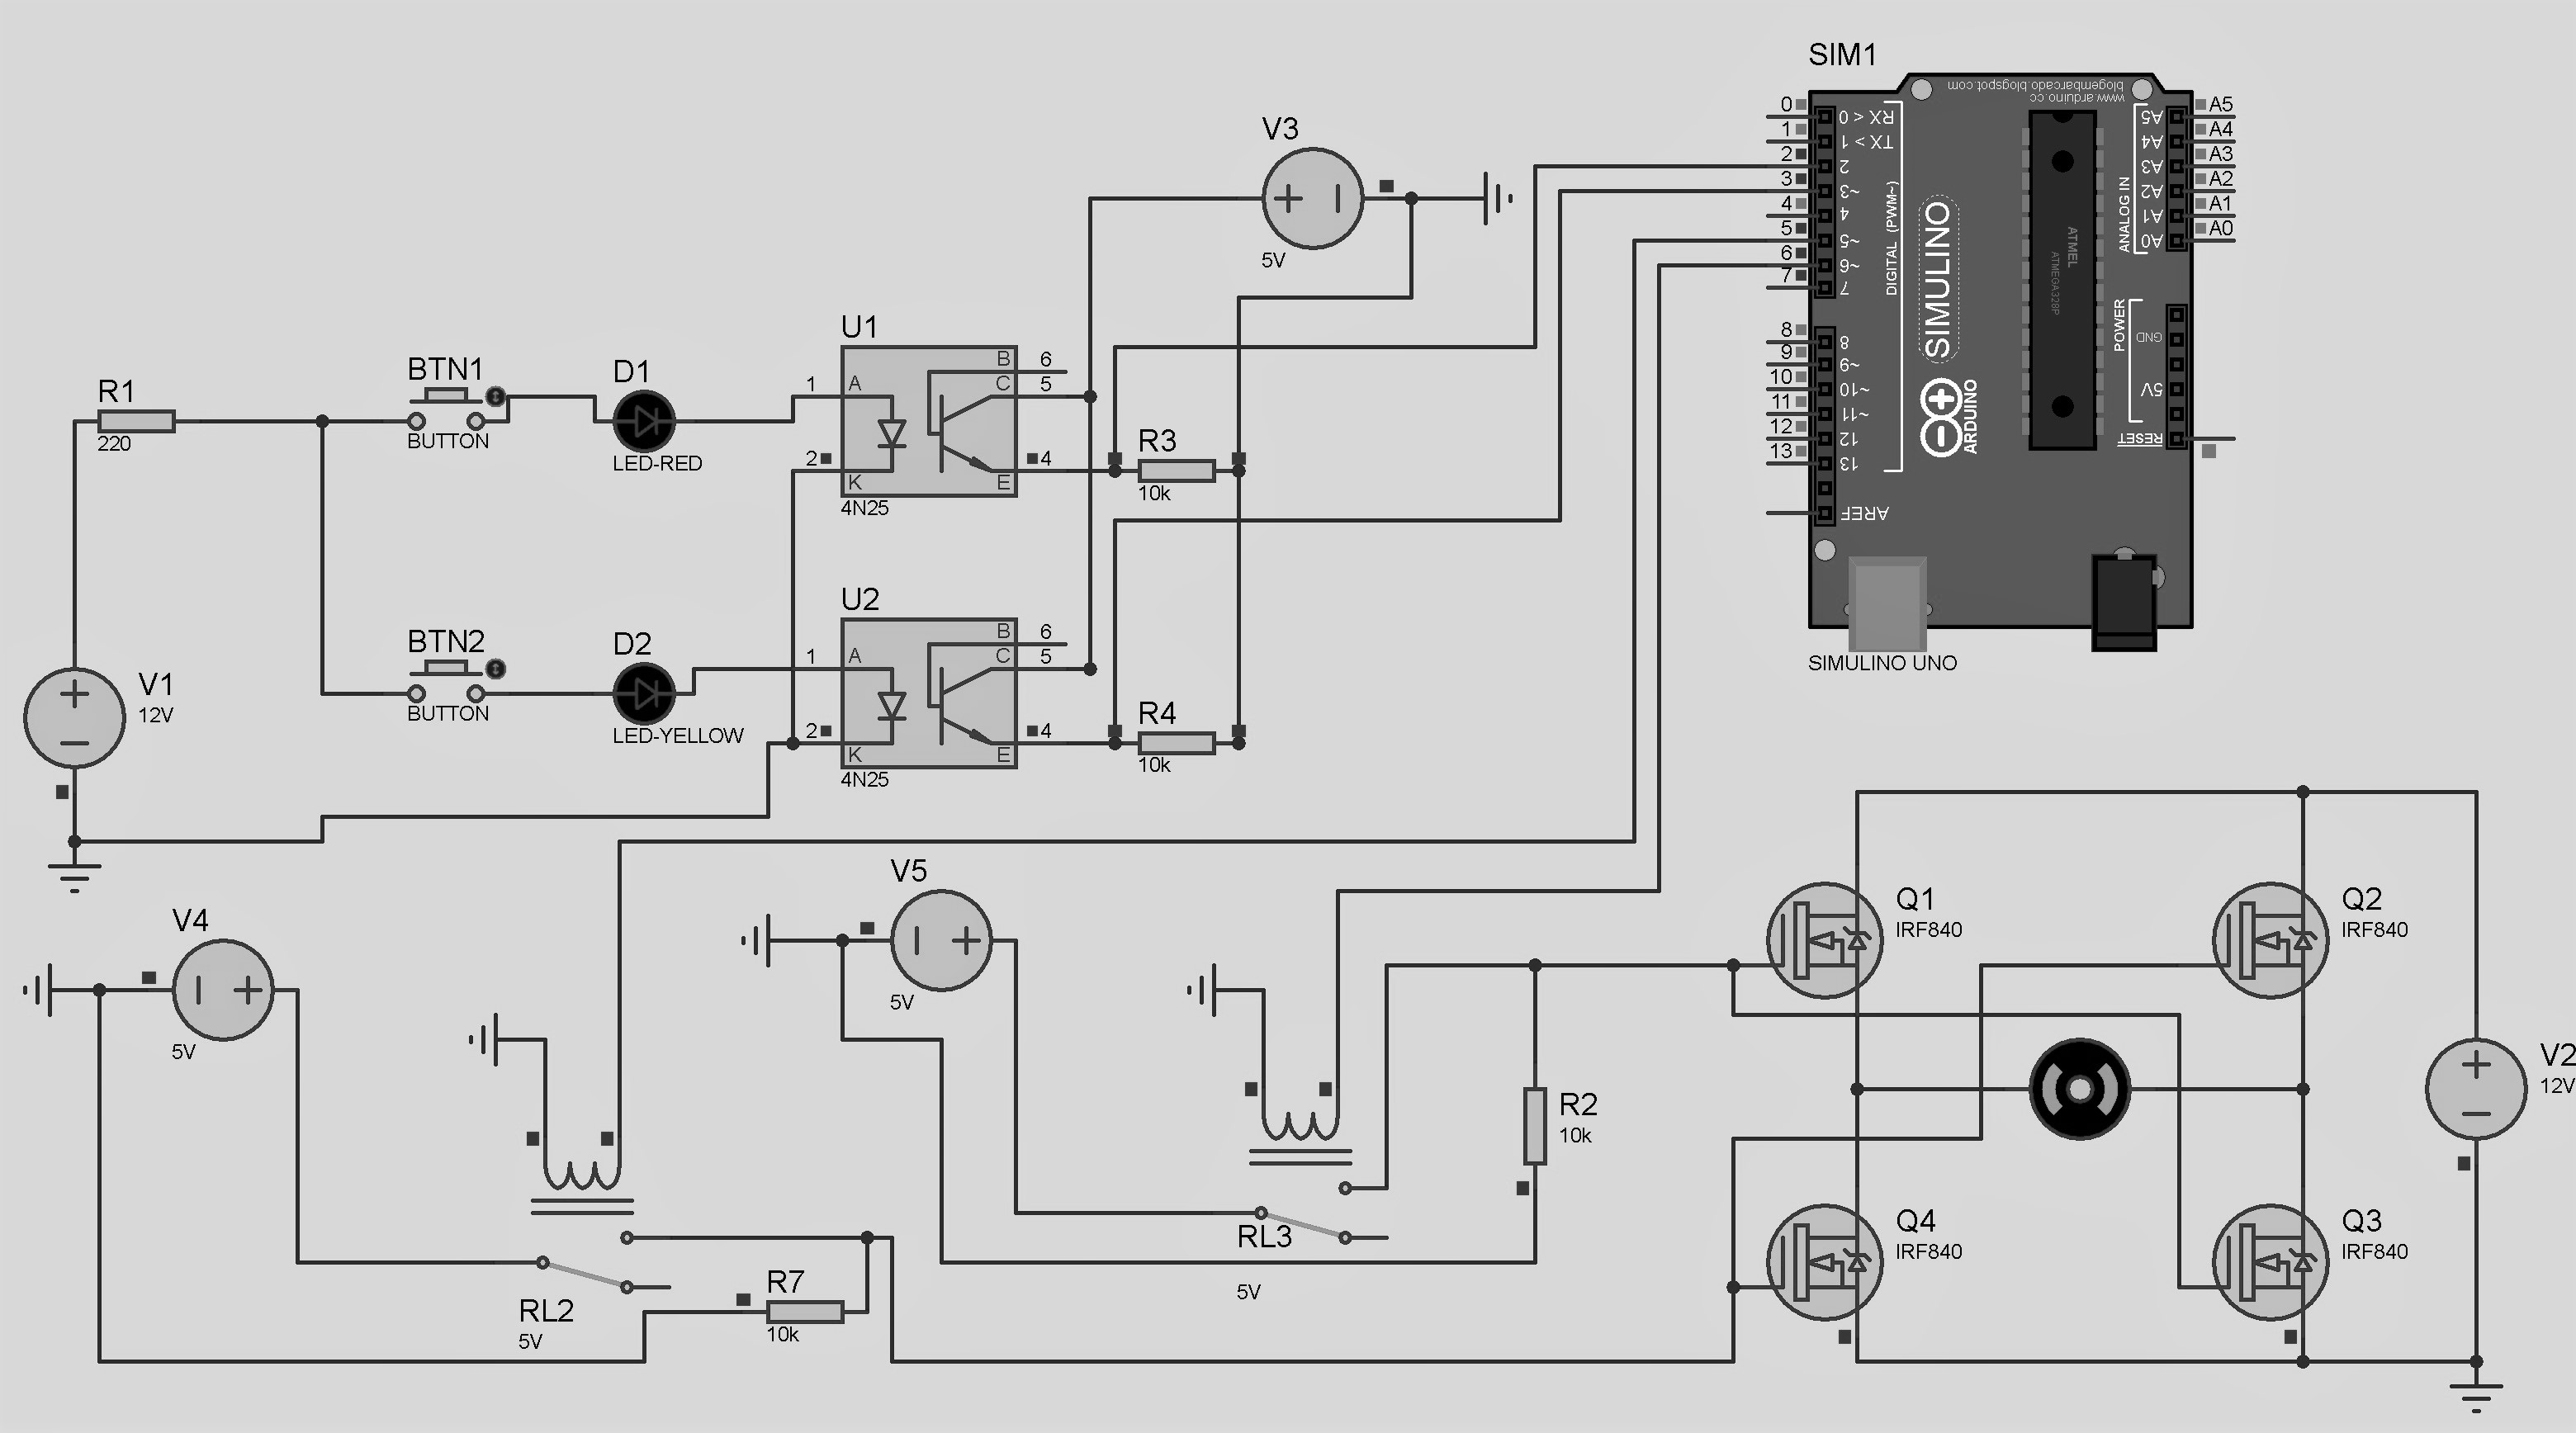
\includegraphics[scale=0.2]{imagenes/circuito.JPG} \linebreak

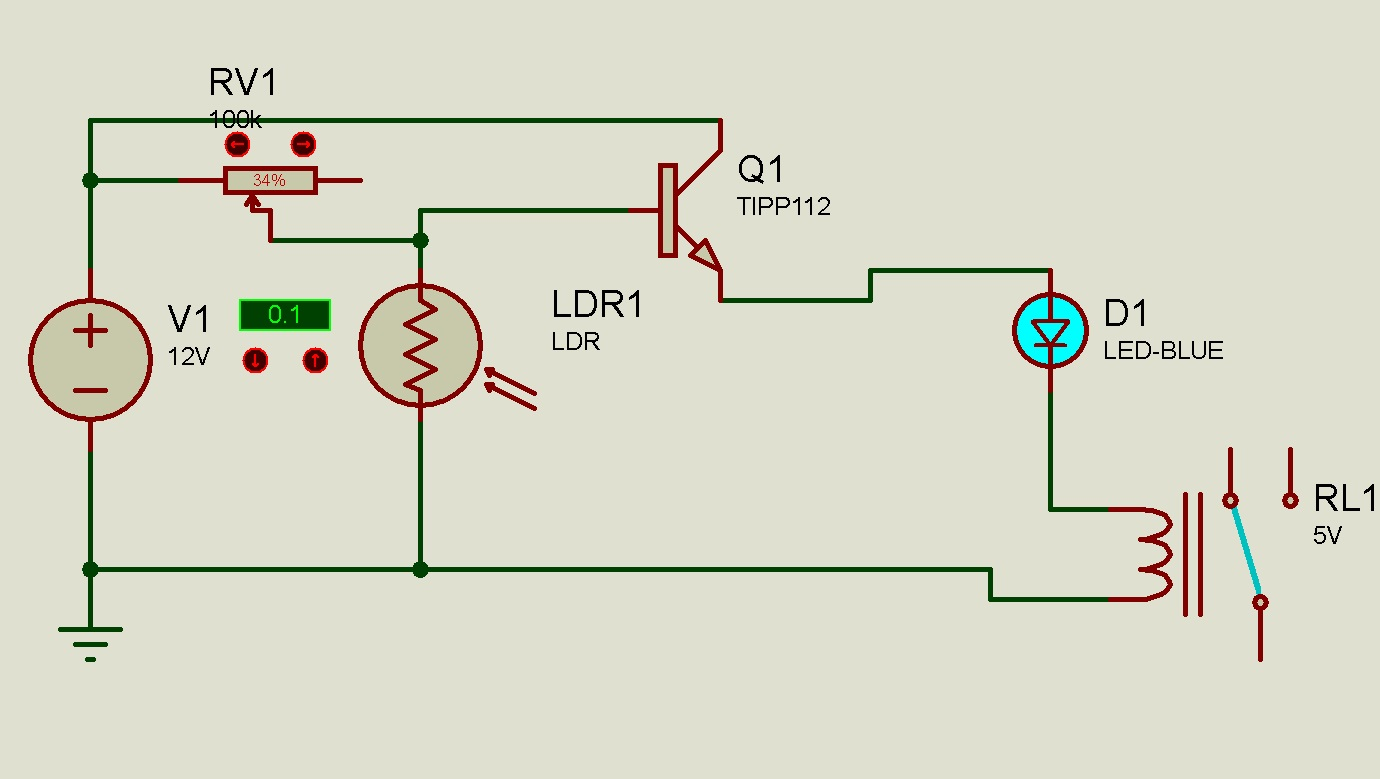
\includegraphics[scale=0.4]{imagenes/circuito0.JPG} \linebreak
\end{center}
\newpage
\begin{flushleft}
\begin{center}
\subsection{Desarrollo de la práctica}
\end{center}
\subsubsection{Parte 1}
Ahora armaremos los circuitos anteriores: \linebreak
\begin{center}
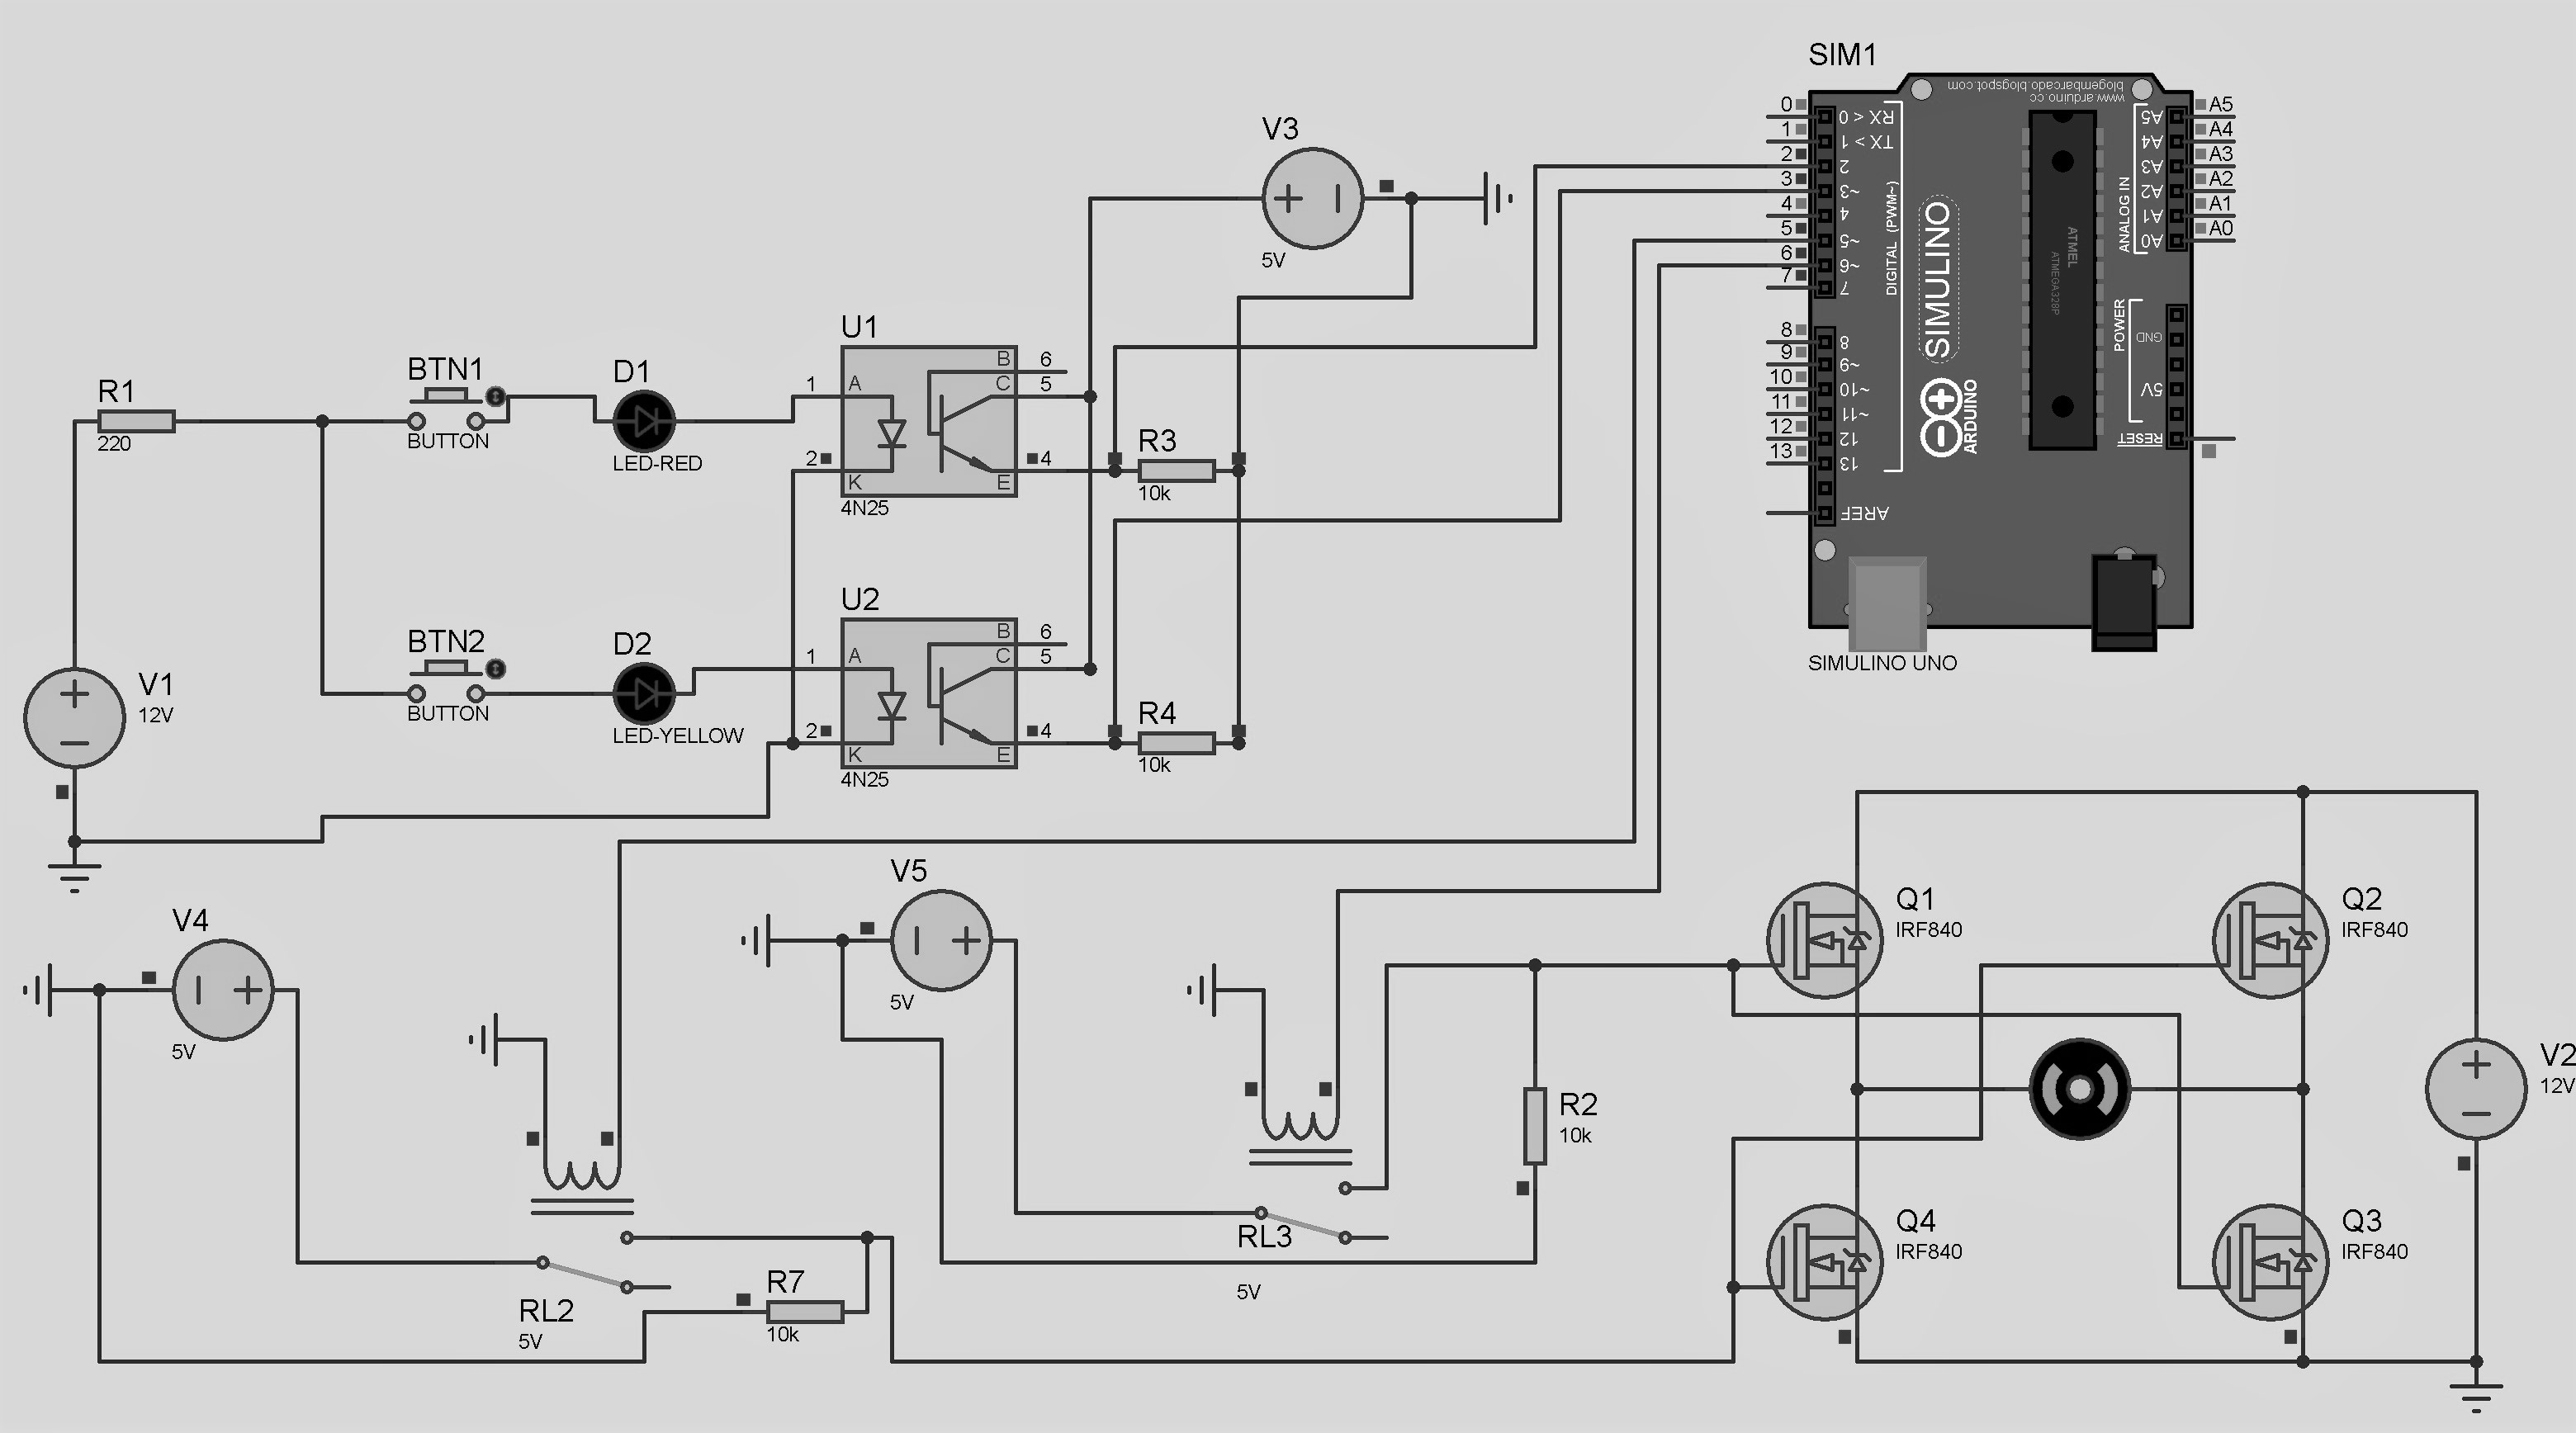
\includegraphics[scale=0.1]{imagenes/circuito.JPG} \linebreak

\end{center}
En este simplemente activaremos lso optoacopladores para asi mandar una señal directamente al arduino y con eso activar la salida hacie nuestro tip 112 es este caso es el transistor darlington a usar y finalmente esto activará el relé y el led, pero la diferencia con practicas anteriores es que puede activar motorea mas potentes como los de un relé industrial.\linebreak

\subsubsection{Parte 2}
En esta parte armaremos un circuito el cual debe ser capaz de activar un led y un relé dependiendo de la luminosidad aplicada a nuestra LDR, cuando iluminemos la LDR la resistencia de esta va a decaer por lo cual perdemos el voltaje necesario para activar la base de nuestro tip 112.\linebreak

\begin{center}
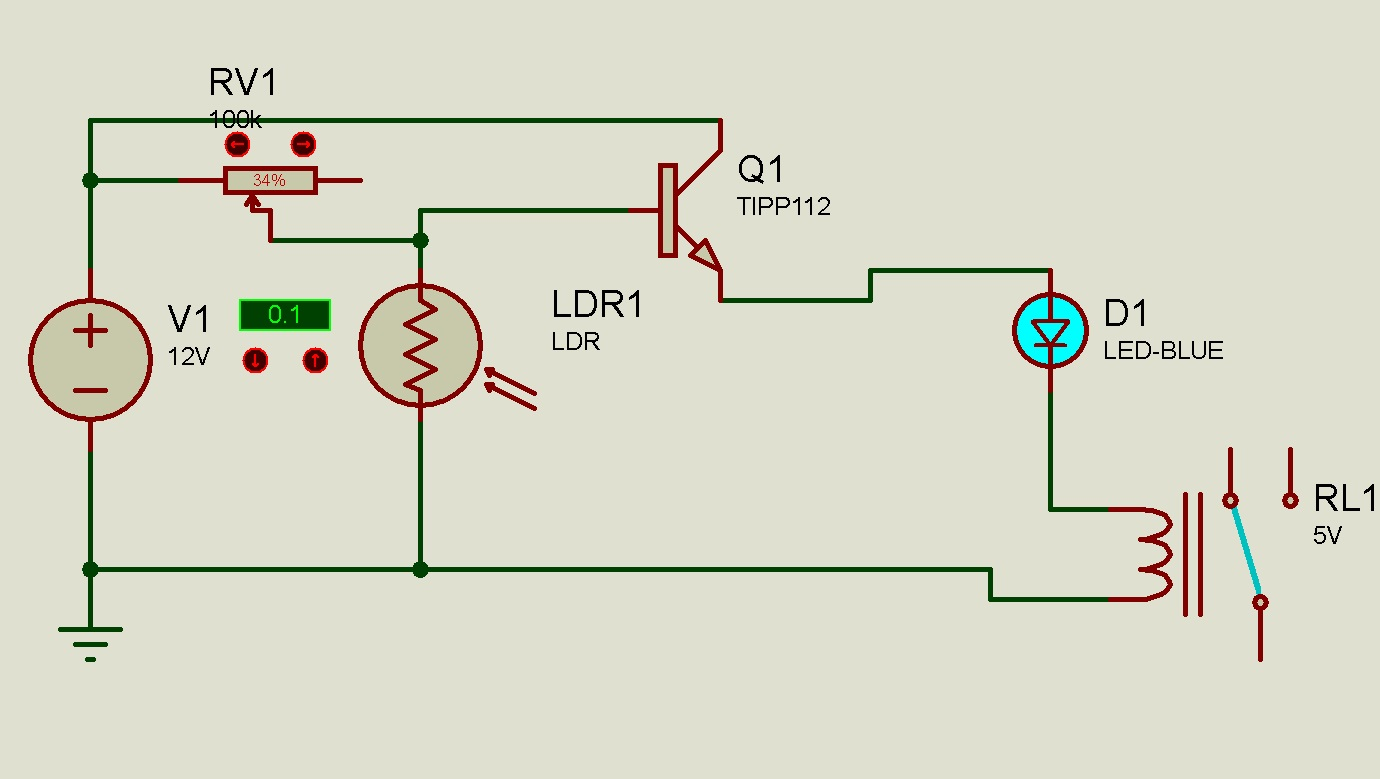
\includegraphics[scale=0.25]{imagenes/circuito0.JPG} \linebreak


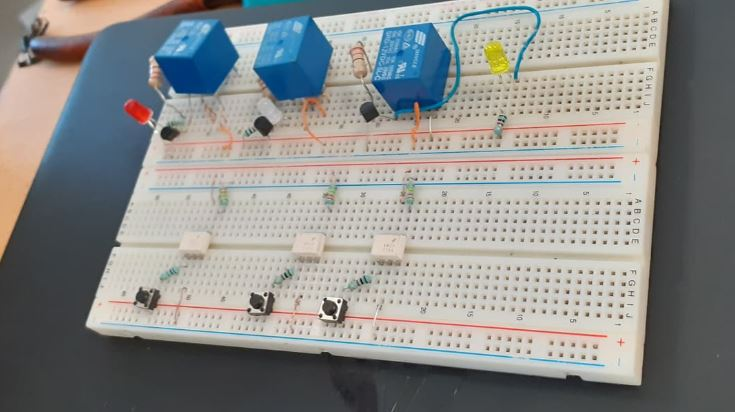
\includegraphics[scale=0.25]{imagenes/circuito1.JPG}
\end{center}
\end{flushleft}
\newpage
\subsection{Conclusiones}
\begin{flushleft}
En esta practica se aprendio el uso de los transistores Darlington los cuales cuentan con caracteristicas extendidas a las de un transistor convencional, esto nos permite relizar el control de circuitos de mayor potencia con la ayuda de estos componentes dada su gran capasidad en cuanto a lo que amperaje refiere incluso podiendo activar motores con consumos de hasta 40w sin problema alguno.
\end{flushleft}
\end{document}

\section{se}